\documentclass{article}
\usepackage[hscale=.85,vscale=.9]{geometry}                % See geometry.pdf to learn the layout options. There are lots.
\geometry{a4paper}                   % ... or a4paper or a5paper or ... 
%\geometry{landscape}                % Activate for for rotated page geometry
%\usepackage[parfill]{parskip}    % Activate to begin paragraphs with an empty line rather than an indent
\usepackage{graphicx}
\usepackage{amssymb}
\usepackage{epstopdf}
\usepackage{lmodern} 
\usepackage{xcolor} 
\DeclareGraphicsRule{.tif}{png}{.png}{`convert #1 `dirname #1`/`basename #1 .tif`.png}
\topmargin=-1.5in
\textheight=12in
\begin{document}
\fontsize{65}{40}\selectfont
\leavevmode
\begin{center}

\sf\bfseries
\textcolor{blue}{The   Game   of   Life}
\vskip -2mm
\fontsize{25}{40}\selectfont
\def\s{\hskip 1.1ex}
\includegraphics[width=1cm]{blend1.png} \s
\includegraphics[width=1cm]{blend2.png} \s
\includegraphics[width=1cm]{blend3.png} \s
\includegraphics[width=1cm]{blend4.png} \s
\includegraphics[width=1cm]{blend5.png} \s
\includegraphics[width=1cm]{blend6.png} \s
\includegraphics[width=1cm]{blend7.png} \s
\includegraphics[width=1cm]{blend8.png} \s
\includegraphics[width=1cm]{blend9.png} \s
\includegraphics[width=1cm]{blend10.png} \\
\includegraphics[width=1cm]{blend11.png} \s
\includegraphics[width=1cm]{blend12.png} \s
\includegraphics[width=1cm]{blend13.png} \s
\includegraphics[width=1cm]{blend14.png} \s
\includegraphics[width=1cm]{blend15.png} \s
\includegraphics[width=1cm]{blend16.png} \s
\includegraphics[width=1cm]{blend17.png} \s
\includegraphics[width=1cm]{blend18.png} \s
\includegraphics[width=1cm]{blend19.png} \s
\includegraphics[width=1cm]{blend20.png}

\fontsize{20}{40}\selectfont
%\vskip -2ex\em Simple rules get surprising effects
\end{center}

\vskip 1cm

\fontsize{14}{16}\selectfont
\def\sec#1{\vskip 3ex\fontsize{18}{16}\selectfont\noindent\textcolor{red}{\textsf{\bfseries #1}}\fontsize{14}{16}\selectfont\noindent}
\def\in{~~~~}
\raggedright
\noindent
When I was 15 I got interested in John Conway's Game of Life reading an article about it in the October 1970 issue of the \emph{Scientific American\/} magazine.

\sec{Computers, free will, and your brain}

%You can imagine Game of Life gliders carrying messages, and indeed people have used them to actually send messages across large game boards, just like sending signals along wires. 

The Game of Life has figured in a lot of arguments about free will. Many people argue the Game of Life has free will because \emph{in principle\/} it is unpredictable. But being unpredictable means the patterns must also be unpredictable \emph{to themselves}, which isn't what I take free will to mean.

\in Although a single brain synapse or neuron can't do much more than a cell in the Game of Life, your amazing brain has around 1,000,000,000,000,000 (1,000 trillion) synapses all working together, ending up with the miraculous complexity of all your memories, your thinking, and your appreciation of science and art.

\in 
With only 150 times more cells than than this exhibit, the Game of Life can simulate 
a fully-working programmable computer. It is a challenging thought that if the Game of Life was scaled up to millions of cells it would be capable of artificial intelligence.

\in One of my favourite examples of how surprising the Game of Life is that the Game of Life can play the Game of Life itself. That is a bit like your consciousness is when you think about yourself, so does that mean the Game of Life can be conscious?

\sec{Very simple rules}

%The Game of Life has simple rules, but very complicated things can happen very quickly. Cells can be `dead' or `alive.' In this display, each live cell is shown by a round stone. 

%\in 
This small exhibit is enough to show how complexity can emerge from simple rules. 

\in Here are \emph{all\/} the rules of the Game of Life: 

\vskip .5cm

\noindent
\def\gap{\hbox to 0in{}}
\begin{tabular}{@{}r@{\hskip 2.5mm}c@{\hskip 2.5mm}p{3.1in}@{\hskip 7mm}}
\textsf{\bfseries Under-population}&--&\sf Any live cell with fewer than two live \hbox{neighbours} dies.\\
\textsf{\bfseries Survival}&--&\sf Any live cell with two or three live \hbox{neighbours} lives on to the next \hbox{generation}.\\
\textsf{\bfseries Reproduction}&--&\sf Three live neighbours reproduce to \hbox{create} a new live cell.\\
\textsf{\bfseries Over-population}&--&\sf Any live cell with more than three live neighbours dies.
\end{tabular}\hskip 0cm\lower .9in\hbox{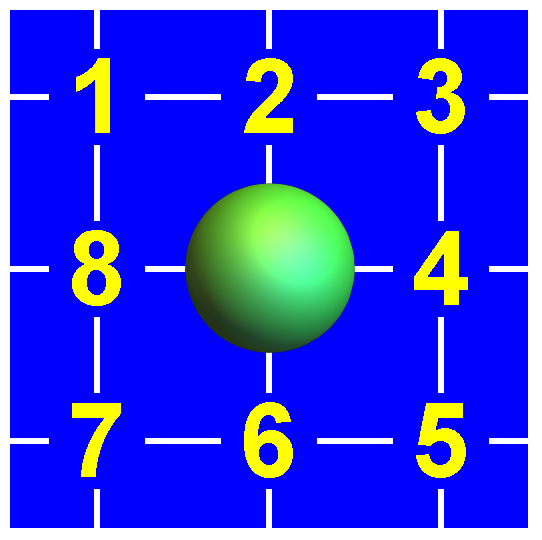
\includegraphics[height=1.9in]{grid.pdf}}
\vskip .5cm

\in That's all there is to it. 

%\in 
%The Game of Life is so popular people spend their time looking for interesting patterns. The display here shows a few popular life forms. Bill Gosper discovered the first ``glider gun'' in 1970 which fires off lots of ``gliders.'' One of Gosper's glider guns is shown at the top of our pre-planned show. You can see it repeatedly shooting gliders diagonally towards the bottom of the display.

\in If you watch the exhibit, you can see how the rules work. The traffic lights (bottom left of the pre-planned show, and often all over the random show) are a good place to appreciate how the simple rules can create action.

\in In the exhibit here the rules are run every fraction of a second to create a new generation, using a Raspberry Pi computer behind the scenes. Newborn cells are green, and as they age they go red then brown, like leaves.

\in Email me, or see the Wikipedia article \emph{Conway's Game of Life} for lots more info.

\vskip 0.8cm
\fontsize{10}{12}\selectfont
\raggedleft
Harold Thimbleby,  June 2026

\texttt{harold@thimbleby.net}


\end{document}  